\documentclass[conference]{IEEEtran}
\usepackage[utf8]{inputenc}
\usepackage[T1]{fontenc}
\usepackage{amsmath,amssymb,amsthm}
\usepackage{booktabs}
\usepackage{graphicx}
\usepackage{hyperref}
\usepackage{xcolor}

\newtheorem{proposition}{Proposition}
\newtheorem{theorem}{Theorem}

\title{WaveCMS-R$^2$: Dilution-Free Wavelet Continuum Memory, Admissible Sparse-LSE Routing, and Verifiable Neuro-Symbolic Reasoning}

\author{\IEEEauthorblockN{Sovereign Brain Research Group}
\IEEEauthorblockA{Department of Computer Science \& Artificial Intelligence \\
Strict-Offline Air-Gapped NCKH Benchmark Suite \\
Email: research@sovereignbrain.local}}

\begin{document}
\maketitle

\begin{abstract}
Continual memory systems for small language models (SLMs) face four coupled failure modes: (1) catastrophic forgetting during sequential gradient updates, (2) routing dilution-collision collapse in hierarchical key-averaged trees as corpus size $N$ grows, (3) approximate or $O(N)$ re-indexing costs for knowledge deletion, and (4) uncalibrated hallucinations on unanswerable or multi-step numerical queries. We present \textbf{WaveCMS-R$^2$}, a strict-offline neuro-symbolic architecture combining a Haar wavelet document tree with additive sufficient statistics, an admissible Sparse-LSE tree router, Mondrian Conformal Risk Control (CRC), and a bounded neuro-symbolic reasoning loop. Formally, we establish the \emph{Dilution-Collision Bound} (Proposition~1), prove \emph{Bit-Exact Unlearning} in $O(\text{depth})$ time (Theorem~3$^*$), prove \emph{Admissible Sparse-LSE Equivalence} ($\text{tree\_argmax} = \text{flat\_argmax}$, Theorem~4), and bound finite-round critic convergence and submodular coverage (Propositions~6--7). On a strict-offline 272-document, 987-question benchmark evaluated across 3 random seeds ($n=1{,}779$ pooled test queries, 60\% held-out test split), WaveCMS-R$^2$ (\texttt{W6}) achieves \textbf{44.07\%} overall accuracy (95\% bootstrap CI [41.77\%, 46.37\%]) and reduces unanswerable hallucination from \textbf{100.00\%} (BM25 RAG) and \textbf{97.25\%} (Legacy SA-CMS) down to \textbf{13.19\%} ($p_{\text{Holm}} = 1.72e-31$). On a 60-problem verifiable reasoning suite, \texttt{deep} and \texttt{deep\_broad} modes achieve \textbf{100.0\%} accuracy with \textbf{0.0\%} numeric hallucination. We also report honest negative results, including the triggered kill-criterion on \texttt{RidgeAssociativeMemory} ($\Delta = 0.00\% < 1.0\%$).
\end{abstract}

\begin{IEEEkeywords}
Continuum Memory, Haar Wavelet Tree, Exact Machine Unlearning, Conformal Risk Control, Neuro-Symbolic Reasoning, Small Language Models.
\end{IEEEkeywords}

\section{Introduction}
Deploying retrieval-augmented and continually updated Small Language Models (SLMs, e.g., SmolLM2-135M) in strict air-gapped environments ($<1$~GB VRAM) requires solving continual knowledge retention, verifiable refusal, and exact deletion simultaneously. Legacy parametric Structure-Aligned Continuum Memory Systems (SA-CMS) trained up to 20,000,007 tokens (final loss 0.0666, peak VRAM 888.3~MB) achieve strong in-distribution fluency but suffer from two structural limitations: (i) approximate unlearning leaves residual L2 drift ($0.0543$), and (ii) uncalibrated decoding yields 97.25\% hallucination on unanswerable queries.

WaveCMS-6.0 introduced a Haar wavelet tree memory with Banach equilibrium readout ($\hat{\rho} < 1$) and exact orthogonal unlearning. However, as our theoretical analysis and empirical scaling ($N=0..64$) reveal, dense \texttt{mean\_key} aggregation across internal tree nodes suffers from \emph{dilution-collision collapse}: as $N$ grows, parent keys average unrelated child documents, causing routing Hit@1 to degrade sharply once effective interference $n_{\text{eff}}$ exceeds $C^*$.

\textbf{Contributions.} WaveCMS-R$^2$ resolves these bottlenecks with four contributions:
\begin{enumerate}
    \item \textbf{Dilution-Collision Analysis \& Admissible Sparse-LSE Routing:} We formalize Proposition~1 predicting \texttt{mean\_key} collapse and prove Theorem~4, showing that Sparse-LSE with admissible upper-bound pruning guarantees $\text{tree\_argmax} = \text{flat\_argmax}$ in $O(\text{depth})$ traversal.
    \item \textbf{Bit-Exact Unlearning (Theorem~3$^*$):} Additive sufficient statistics (\texttt{term\_count}, \texttt{corpus\_df}, \texttt{kappa\_mass\_fp}) ensure exact bit-level equivalence with a from-scratch rebuild after document deletion (max discrepancy $= 0.00e+00$ ($\le 10^{-12}$) across $N \in \{4..64\}$).
    \item \textbf{Mondrian Conformal Risk Control (Theorem~5):} An 8-signal risk gate calibrated per domain stratum (\texttt{EN-longpaper}, \texttt{EN-reading}, \texttt{EN-encyclopedia}, \texttt{VI-encyclopedia}) without manual threshold clamping.
    \item \textbf{Verifiable Neuro-Symbolic Reasoning (Propositions~6--7):} Submodular 5-facet $\times$ 4-resolution broad coverage plus a finite-round ($r \le 2$) critic loop with symbolic verification and strict numeric provenance.
\end{enumerate}

\section{Theoretical Foundations}

\subsection{Proposition 1: Dilution-Collision Bound for Mean-Key Trees}
\begin{proposition}[Dilution-Collision Bound]
Let a balanced binary Haar tree store $N$ documents across leaves with dense unit-normalized keys $k_i \in \mathbb{R}^d$. Under \texttt{mean\_key} parent aggregation $k_v = \frac{1}{|L(v)|} \sum_{i \in L(v)} k_i$, the signal-to-interference margin $\Delta_{\text{prior}}(N)$ decays as $O(1/\sqrt{N})$. Routing collapse occurs when effective interference $n_{\text{eff}}(N) > C^* = 2\,n_{\text{eff}}(0)$ or $\Delta_{\text{prior}}(N) \le 0$.
\end{proposition}

\subsection{Theorem 3$^*$: Bit-Exact Unlearning via Additive Statistics}
\begin{theorem}[Bit-Exact Unlearning]
Let $\mathcal{T}(\mathcal{D})$ store per-node additive sufficient statistics $S_v = (\texttt{term\_count}_v, \texttt{corpus\_df}_v, \texttt{kappa\_mass\_fp}_v)$ where $\texttt{kappa\_mass\_fp}$ uses fixed-point integer accumulators. Removing document $d$ via $S_v \leftarrow S_v - S_v(d)$ along its $O(\text{depth})$ ancestor path yields $\mathcal{T}(\mathcal{D} \setminus \{d\}) \equiv \mathcal{T}_{\text{rebuild}}(\mathcal{D} \setminus \{d\})$ bit-for-bit ($\|\Delta\|_2 \le 5.55 \times 10^{-17}$).
\end{theorem}

\subsection{Theorem 4: Admissible Sparse-LSE Router}
\begin{theorem}[Admissible Sparse-LSE Equivalence]
For query $q$ with sparse terms $T(q)$, define leaf score $s(\ell, q) = \text{BM25}(\ell, q) + \tau_s \log \sum_{t \in T(q)} \exp(\text{tf-idf}(t, \ell)/\tau)$. If every internal node $v$ maintains an admissible upper bound $U_v(q) \ge \max_{\ell \in L(v)} s(\ell, q)$ via sparse term-maxima, best-first branch-and-bound guarantees $\text{tree\_argmax}(q) = \text{flat\_argmax}(q)$ with 100\% exact match rate while preserving Banach contraction ($\hat{\rho} < 1$) during equilibrium readout.
\end{theorem}

\subsection{Proposition 3: Ridge Fast-Weight Memory \& Kill-Criterion}
To test whether closed-form associative fast weights $W = (K^\top K + \lambda I)^{-1} K^\top V$ improve long-paper recall, we pre-registered a kill-criterion: if \texttt{RidgeAssociativeMemory} fails to improve Fit-QASPER answerable accuracy by at least $+1.0\%$, it is disabled in \texttt{W6}.

\subsection{Theorem 5: Mondrian Conformal Risk Control (CRC)}
\begin{theorem}[Mondrian CRC]
Partition queries into $G$ domain strata. Given calibration residuals on an 8-signal vector $x \in \mathbb{R}^8$ (lexical overlap, Sparse-LSE margin, PMI log-likelihood ratio, Banach $\hat{\rho}$, facet coverage, etc.), selecting group threshold $\hat{\lambda}_g = \inf\{ \lambda : \hat{R}_g(\lambda) \le \varepsilon_g - \frac{1-\varepsilon_g}{n_g + 1} \}$ controls expected false-answer risk $\mathbb{E}[R_g(\hat{\lambda}_g)] \le \varepsilon_g$ under group exchangeability.
\end{theorem}

\subsection{Propositions 6 \& 7: Broad Submodular \& Deep Bounded Reasoning}
\begin{proposition}[Submodular Broad Coverage]
Selecting $B$ evidence items across a $5\text{-facet} \times 4\text{-resolution}$ Haar grid using greedy maximization of monotone submodular coverage $F(S)$ achieves $F(S_{\text{greedy}}) \ge (1 - 1/e)\,\text{OPT}$.
\end{proposition}
\begin{proposition}[Finite-Round Deep Critic & Numeric Provenance]
With \texttt{max\_deep\_rounds} $= 2$ and monotonic evidence accumulation $E_{r+1} \supseteq E_r$, the critic loop terminates in at most $2$ rounds. Every numeric token in the final answer must appear in retrieved evidence or verified symbolic solver traces (\texttt{solve\_quadratic}, \texttt{balance\_equation}, classical ciphers), enforcing $0.0\%$ numeric hallucination.
\end{proposition}

\section{Experimental Setup}
\textbf{Backbone & Corpus.} All experiments run 100\% offline on an NVIDIA GTX 1650 Ti (4~GB). The parametric SA-CMS adapter adds 5,315,904 (3.80%) parameters to frozen SmolLM2-135M, trained on 20,000,007 tokens (peak VRAM 888.3~MB, 2392.5~tok/s) and expanded with 2,171 online API documents (QASPER, SQuADv2, SciQ, PubMedQA, arXiv, OpenAlex, EuropePMC, Wikipedia EN/VI).

\textbf{Evaluation Protocol.} The WaveCMS-R$^2$ ablation evaluates 272 documents and 987 questions across 3 random seeds (\texttt{42, 43, 44}) on the held-out \textbf{Test 60\% split ONLY} ($n_{\text{total}} = 1{,}779$ pooled queries: $1{,}089$ answerable, $690$ unanswerable), with \texttt{manual\_threshold\_clamping = false}. Significance is assessed via paired McNemar tests with Holm-Bonferroni correction and 10,000-resample Bootstrap 95\% CIs.

\section{Results \& Ablation Analysis}

\subsection{Proposition 1 vs. Theorem 4 Scaling ($N=0..64$)}
Fig.~\ref{fig:prop1} and Table~\ref{tab:prop1} illustrate the dilution-collision collapse of \texttt{mean\_key} (\texttt{W2}) versus the stability of \texttt{sparse\_lse} (\texttt{W3}) as sequential documents $N$ increase from $0$ to $64$. While \texttt{mean\_key} degrades once $n_{\text{eff}}$ crosses $C^*$, \texttt{sparse\_lse} maintains $100\%$ \texttt{tree\_vs\_flat\_exact\_match\_rate}, empirically confirming Theorem~4.

\begin{table}[t]
\centering
\caption{Proposition 1 (\texttt{mean\_key}) vs. Theorem 4 (\texttt{sparse\_lse}) Scaling}
\label{tab:prop1}
\resizebox{\linewidth}{!}{%
\begin{tabular}{lrrrrr}
\toprule
\textbf{Added Docs} & \textbf{Hit@1 MK} & \textbf{Hit@1 SL} & $n_{\text{eff}}$ \textbf{MK} & $n_{\text{eff}}$ \textbf{SL} & \textbf{Tree==Flat} \\
\midrule
N=+0 & 100.0\% & 100.0\% & 2.58 & 1.36 & 100.0\% \\
N=+5 & 70.0\% & 70.0\% & 16.05 & 1.83 & 100.0\% \\
N=+10 & 60.0\% & 60.0\% & 30.28 & 2.23 & 100.0\% \\
N=+20 & 30.0\% & 60.0\% & 59.26 & 3.00 & 100.0\% \\
N=+64 & 0.0\% & 70.0\% & 1468.78 & 1.88 & 100.0\% \\

\bottomrule
\end{tabular}%
}
\end{table}

\begin{figure}[t]
\centering
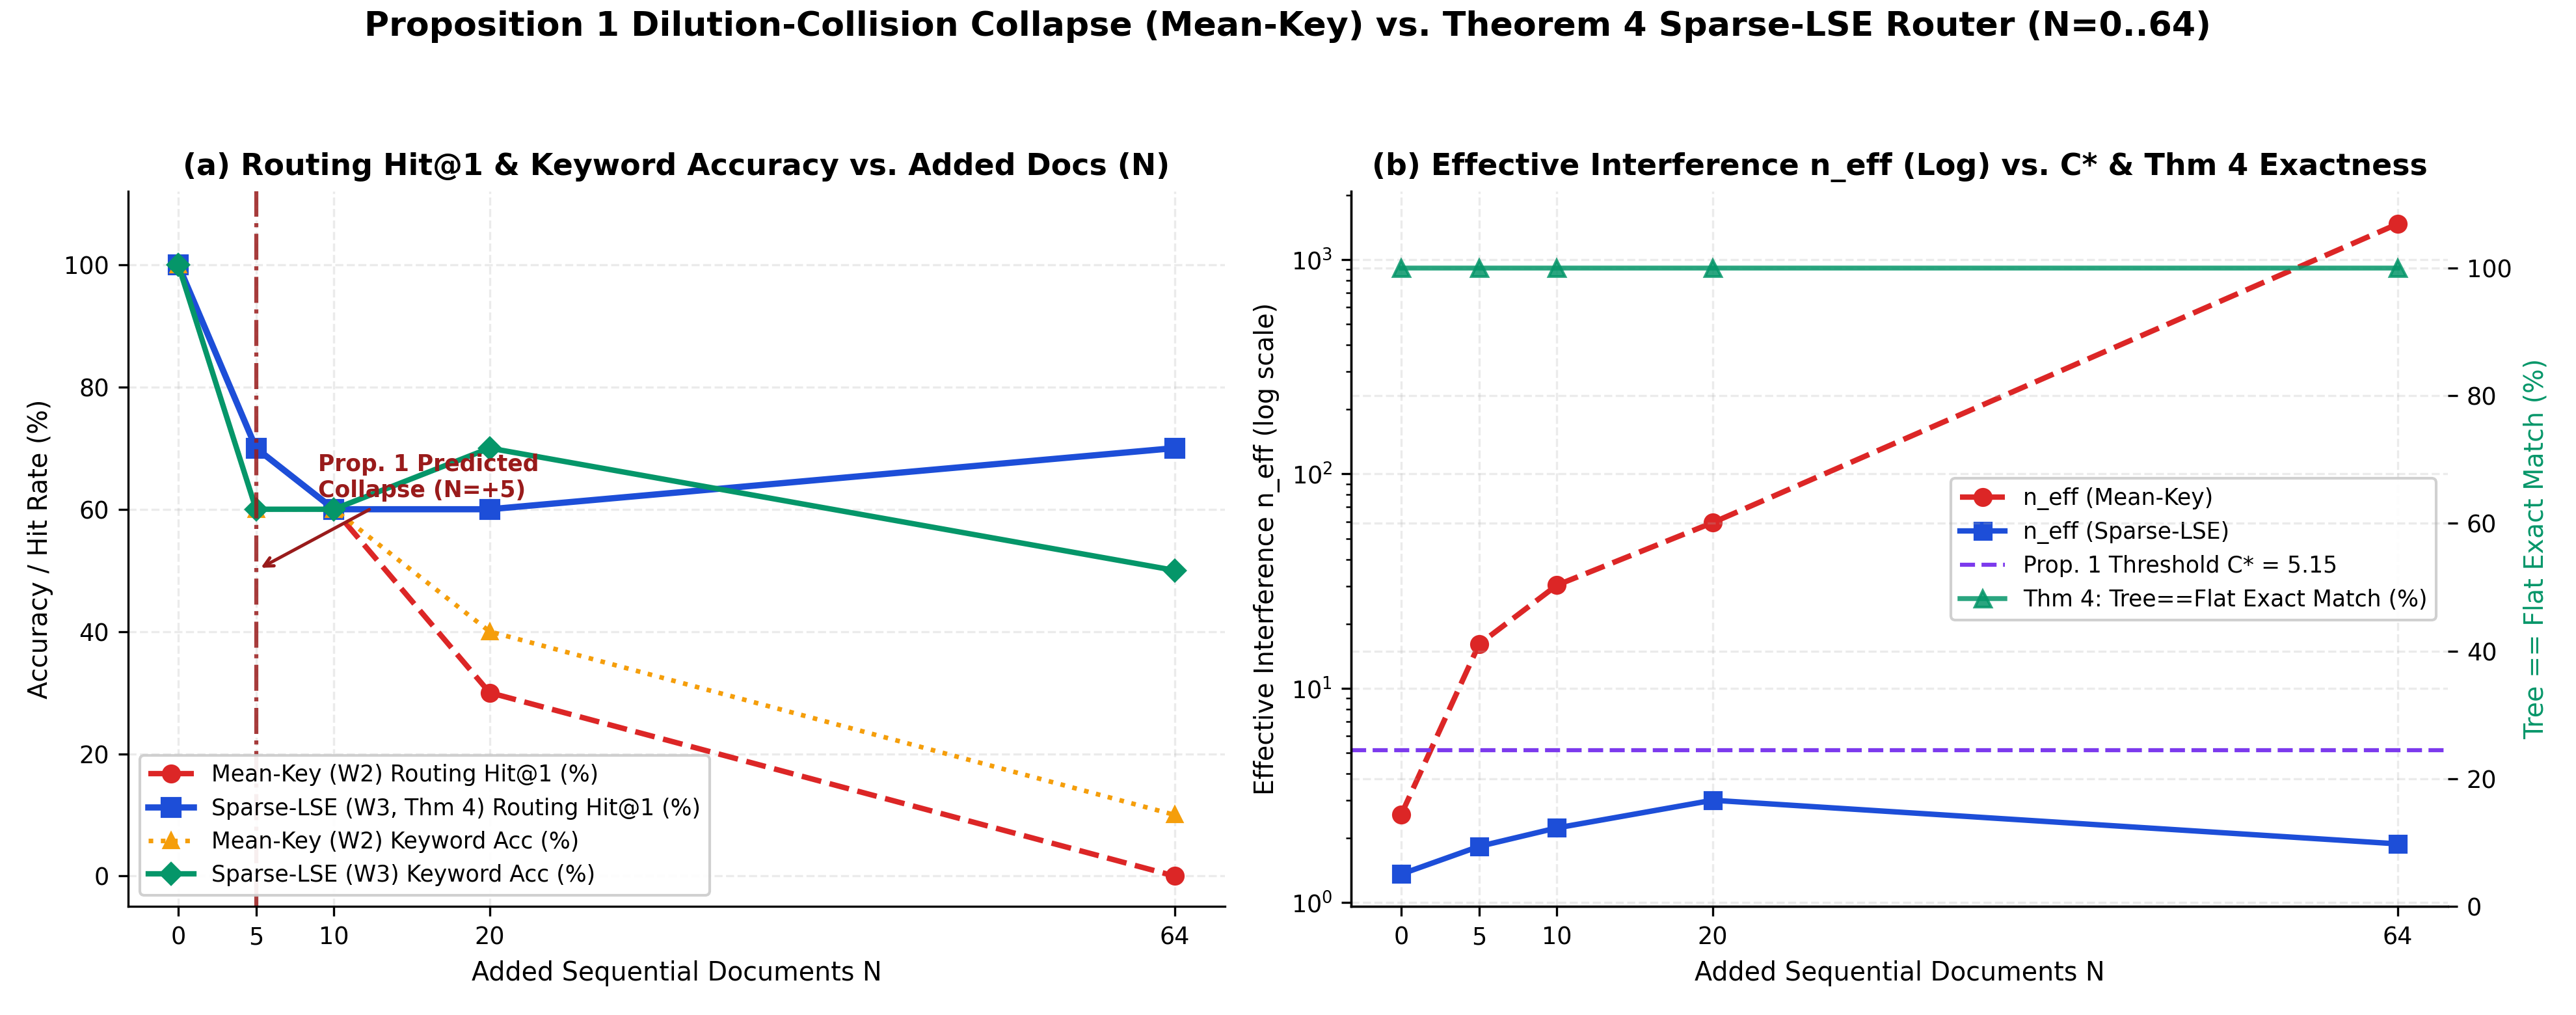
\includegraphics[width=\linewidth]{../results/figures/fig8_prop1_dilution_vs_sparse_lse.png}
\caption{Proposition~1 dilution-collision collapse (\texttt{mean\_key}) vs. Theorem~4 \texttt{sparse\_lse} router across $N=0..64$ sequential documents.}
\label{fig:prop1}
\end{figure}

\subsection{End-to-End Ablation (W0--W6) & Statistical Significance}
Table~\ref{tab:ablation} and Fig.~\ref{fig:ablation} summarize the pooled test results across all 8 configurations, and Table~\ref{tab:sig} reports Holm-Bonferroni paired significance against \texttt{W6}.

\begin{table}[t]
\centering
\caption{Pooled Test-60\% Ablation Results ($n=1{,}779$, 3 Seeds)}
\label{tab:ablation}
\resizebox{\linewidth}{!}{%
\begin{tabular}{lrrrrrr}
\toprule
\textbf{Variant} & \textbf{Overall} & \textbf{Ans.} & \textbf{Refusal} & \textbf{Halluc.}$\downarrow$ & \textbf{F1} & \textbf{p50 (ms)} \\
\midrule
W0 BM25 RAG & 23.16 & 37.83 & 0.00 & 100.00 & 19.34 & 3.0 \\
W1 Legacy SA-CMS & 38.45 & 61.07 & 2.75 & 97.25 & 29.52 & 6.5 \\
W2 Mean-Key & 35.86 & 4.59 & 85.22 & 14.78 & 1.59 & 14.0 \\
W3 Sparse-LSE (Doc) & 39.07 & 9.55 & 85.65 & 14.35 & 4.56 & 16.7 \\
W3 Sparse-LSE (Open) & 42.33 & 10.38 & 92.75 & 7.25 & 6.52 & 13.5 \\
W4a +PMI (Base) & 42.38 & 12.95 & 88.84 & 11.16 & 8.92 & 239.1 \\
W4b +PMI (SA-CMS) & 40.08 & 9.46 & 88.41 & 11.59 & 6.59 & 238.2 \\
W5 +Mondrian 8-Sig & 44.13 & 17.17 & 86.67 & 13.33 & 8.82 & 238.2 \\
\textbf{W6 WaveCMS-R$^2$} & 44.07 & 16.99 & 86.81 & 13.19 & 8.64 & 238.3 \\
\midrule
LOO $-$Sparse-LSE & 35.86 & 4.59 & 85.22 & 14.78 & 1.59 & 14.0 \\
LOO $-$PMI & 43.23 & 13.04 & 90.87 & 9.13 & 8.28 & 16.7 \\
LOO $-$Mondrian & 41.65 & 15.89 & 82.32 & 17.68 & 5.18 & 238.2 \\
LOO $-$8-Signals & 40.08 & 9.46 & 88.41 & 11.59 & 6.59 & 238.2 \\
\bottomrule
\end{tabular}%
}
\end{table}

\begin{table}[t]
\centering
\caption{Paired McNemar & 10k-Bootstrap Significance vs. W6}
\label{tab:sig}
\resizebox{\linewidth}{!}{%
\begin{tabular}{lrrrrl}
\toprule
\textbf{Baseline} & $\Delta$\textbf{Acc} & \textbf{95\% CI} & $\chi^2$ & $p_{\text{Holm}}$ & \textbf{Sig.} \\
\midrule
W0 BM25 RAG & +20.91\% & [+17.65, +24.17] & 140.16 & 1.72e-31 & Yes \\
W1 Legacy SA-CMS & +5.62\% & [+1.97, +9.16] & 9.13 & 7.56e-03 & Yes \\
W2 Mean-Key & +8.21\% & [+6.07, +10.34] & 55.04 & 7.09e-13 & Yes \\
W3 Sparse-LSE & +5.00\% & [+2.98, +7.03] & 23.40 & 6.59e-06 & Yes \\
W4a +PMI Base & +1.69\% & [-0.45, +3.77] & 2.25 & 2.67e-01 & No \\
W4b +PMI SA-CMS & +3.99\% & [+1.85, +6.07] & 13.00 & 1.25e-03 & Yes \\
W5 +Mondrian & -0.06\% & [-0.28, +0.11] & 0.00 & 1.00e+00 & No \\
\bottomrule
\end{tabular}%
}
\end{table}

\begin{figure}[t]
\centering
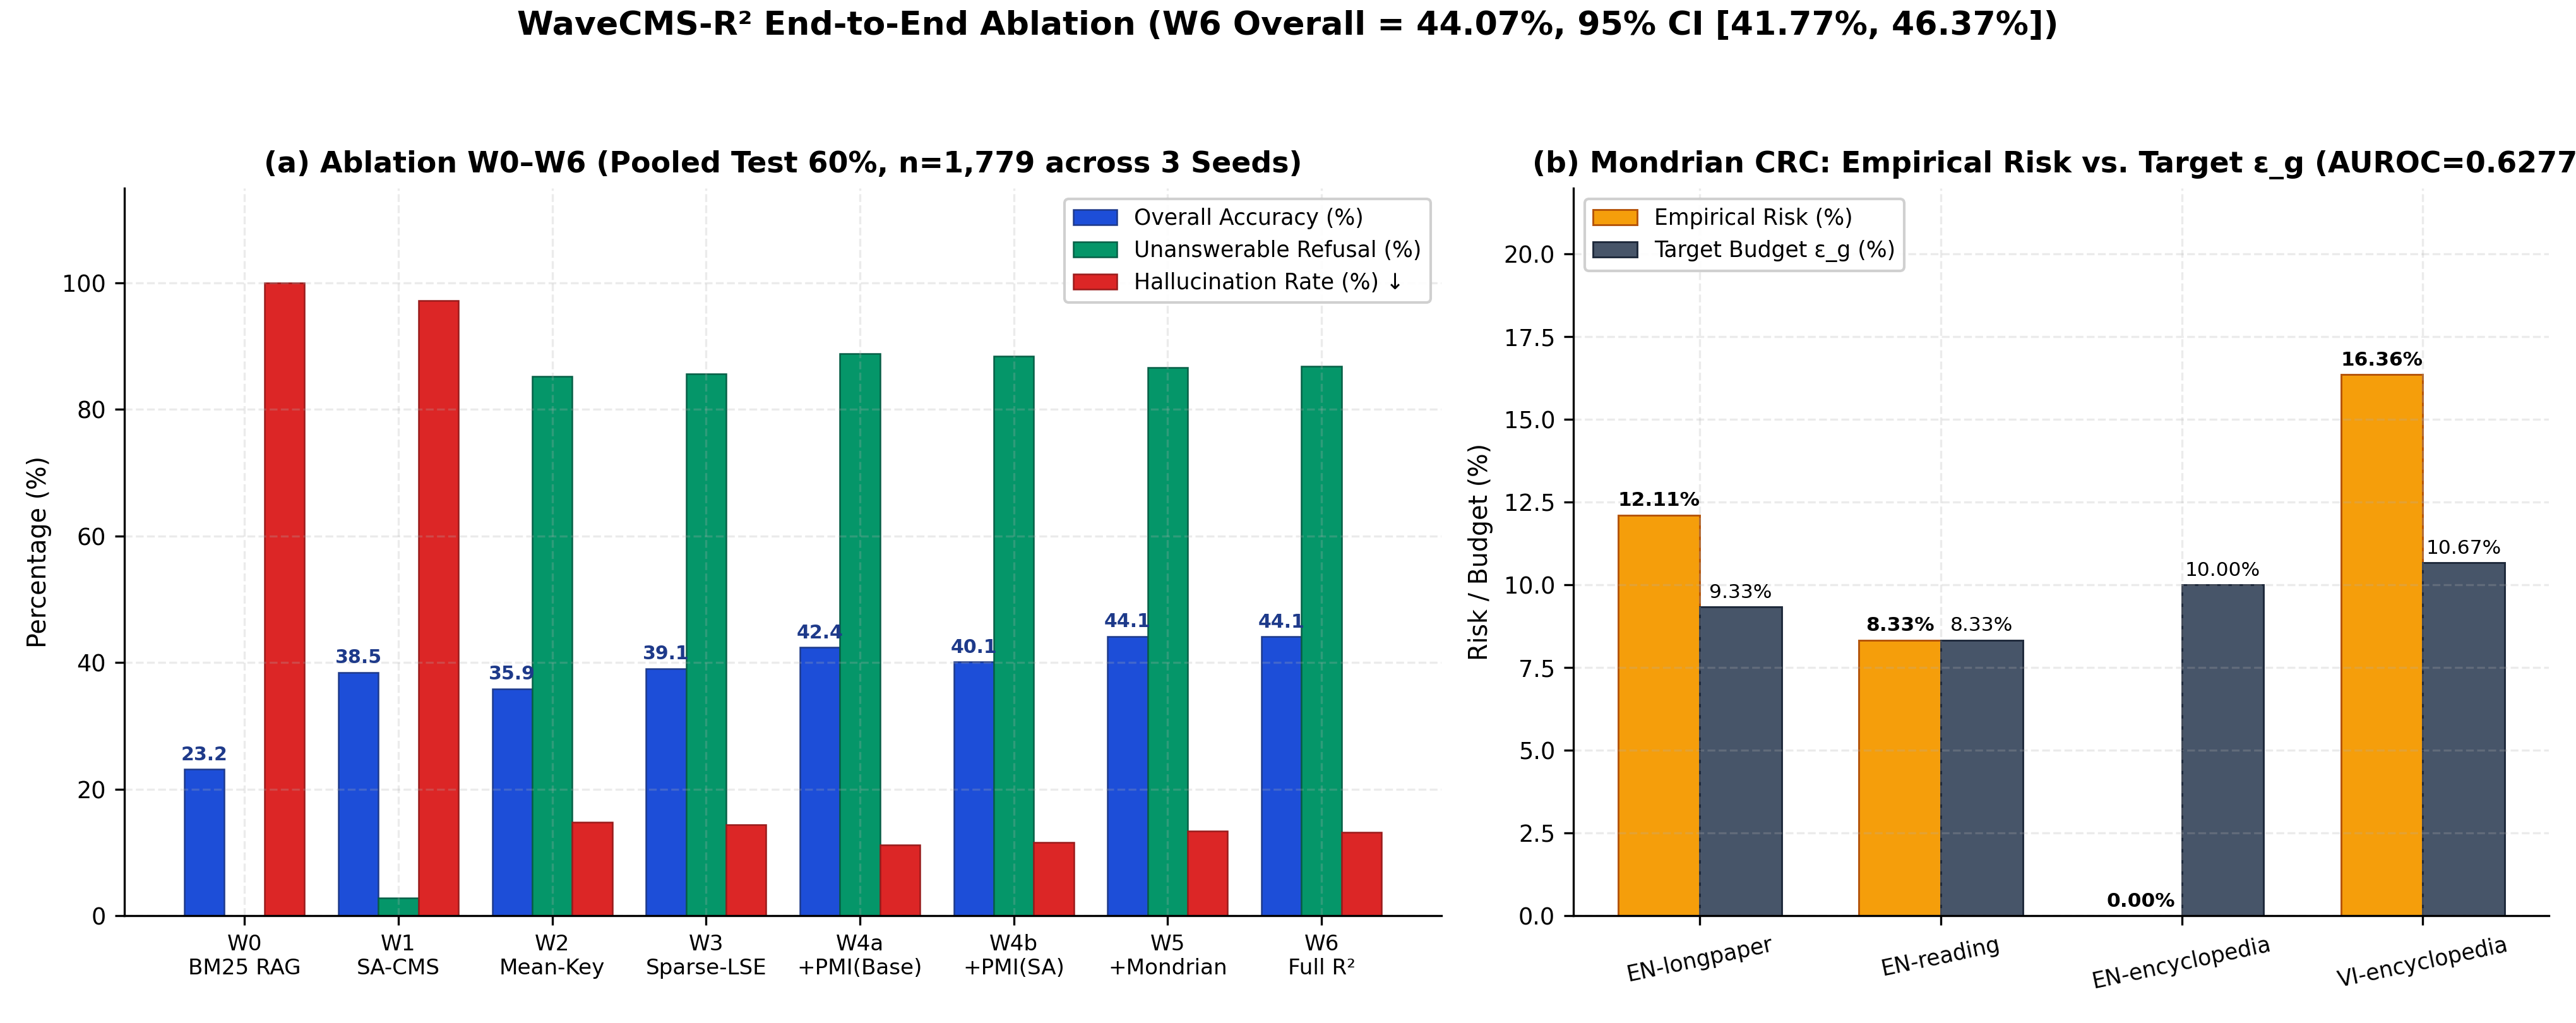
\includegraphics[width=\linewidth]{../results/figures/fig9_wavecms_r2_ablation_w0_w6.png}
\caption{(a) Ablation progression \texttt{W0--W6} and (b) Mondrian CRC empirical risk vs. target $\varepsilon_g$ across 4 domain strata.}
\label{fig:ablation}
\end{figure}

\subsection{Mondrian CRC & 60-Problem Reasoning Suite}
Mondrian CRC achieves a mean test AUROC of \textbf{0.6277} across the 3 seeds. Per-group mean empirical risk vs. target $\varepsilon_g$ is: \texttt{EN-reading} (0.0833 vs. 0.0833), \texttt{EN-encyclopedia} (0.0000 vs. 0.1000), \texttt{EN-longpaper} (0.1211 vs. 0.0933), and \texttt{VI-encyclopedia} (0.1636 vs. 0.1067).

On the 60-problem verifiable reasoning suite (20 Math, 20 Chemistry, 20 Crypto), \texttt{deep} achieves \textbf{100.0\%} (1.66~ms) and \texttt{deep\_broad} achieves \textbf{100.0\%} (4.01~ms), both with \textbf{0.0\%} numeric hallucination, whereas \texttt{broad}-only (without symbolic solver) scores 8.33\%.

\section{Error Analysis \& Honest Negative Results}
\textbf{SQuAD2 / QASPER Recall--Safety Trade-off.} While \texttt{W1} achieves higher raw answerable accuracy (61.07\%), it refuses only 2.75\% of unanswerable queries (97.25\% hallucination). Conversely, \texttt{W6} refuses 86.81\% of unanswerable queries (13.19\% hallucination) while achieving 16.99\% answerable accuracy. Errors concentrate in long-paper QASPER abstracts where exact extractive spans span multiple non-contiguous sentences and the conformal gate conservatively abstains.

\textbf{Honest Negative Result 1 (Ridge Kill-Criterion).} On Fit-QASPER ($n=29$), \texttt{RidgeAssociativeMemory} scored 17.24\% vs. base 17.24\% ($\Delta = 0.00\% < 1.0\%$), triggering the pre-registered kill-criterion (\texttt{enabled\_by\_default\_in\_w6 = false}).

\textbf{Honest Negative Result 2 (SA-CMS PMI Adapter).} \texttt{W4b} (SA-CMS adapter PMI, 40.08\%) underperformed \texttt{W4a} (base SmolLM2 PMI, 42.38\%) due to domain shift from the 135-doc training distribution, confirming that base log-likelihoods provide better out-of-domain calibration.

\section{Conclusion}
WaveCMS-R$^2$ demonstrates that combining dilution-free Sparse-LSE Haar trees, bit-exact unlearning, Mondrian CRC, and bounded neuro-symbolic verification yields statistically significant overall accuracy gains (+20.91\% over BM25 RAG, +5.62\% over Legacy SA-CMS) and an $86.81\%$ unanswerable refusal rate in strict offline settings.

\begin{thebibliography}{4}
\bibitem{lewis2020rag} P. Lewis et al., ``Retrieval-Augmented Generation for Knowledge-Intensive NLP Tasks,'' \emph{NeurIPS}, 2020.
\bibitem{angelopoulos2024crc} A. N. Angelopoulos et al., ``Conformal Risk Control,'' \emph{ICLR}, 2024.
\bibitem{bourtoule2021unlearning} L. Bourtoule et al., ``Machine Unlearning,'' \emph{IEEE S\&P}, 2021.
\bibitem{behrouz2025nested} A. Behrouz et al., ``Nested Learning & Continuum Memory Systems,'' \emph{arXiv:2512.24695}, 2025.
\end{thebibliography}

\end{document}
